\section{Distributed MSI}
\label{sec:DistributedMsi}

We will take the protocol designer's perspective, and first describe what the
designer has to specify to create a distributed protocol.

Each cache can only read and write its local state. A cache maintains a shadow
 of all its children's states in the form of a directory. The designer can
always assume that the state of an actual child is what is given in the
directory. The directory entry of address $a$ for $this$' child $c$ is denoted
using $this.dir[c][a]$.

The designer has to specify the handlers for \uReq{} and \dReq{}. In the
following, we assume that the cache whose handler the designer is writing is
$this$ and the relevant address is $a$.

In order to read a child's state, the designer simply reads the state of the
directory for that child. But to modify the state of child $c$ to $x$, the
designer specifies a command \send{} \Req{this}{c}{a}{x}, followed by \receive{}
\Resp{c}{this}{a}{y}. Command \send{} \Req{this}{c}{a}{x} can be called only when $x
< this.dir[c][a]$. $y$ denotes a free variable which gets filled with the value of
the state $c$ has changed to. $y$ is guaranteed to be $\le x$. $this.dir[c][a]$
should be updated with this value.

In order to read the data of another node $n$ (parent or child),
the designer issues the command \receive{} \Data{this}{n}{a}{d}, where $d$ is a free
variable that gets filled with the data. To write the data into address $a$ of
another node $n$ (parent or child), the designer issues the command \send{}
\Data{this}{n}{a}{this.data[a]}.

In order to upgrade the state of $this$ to $x$, the designer has to
specify the command \send{} \Req{this}{p}{a}{x} followed by \receive{}
\Resp{p}{this}{a}{y}. Command \send{} \Req{this}{p}{a}{x} can be called only when $x
> this.state[x]$. $y$ denotes a free variable which gets filled with the value of
the state $this$ should be upgraded to. $y$ is guaranteed to be $\ge x$.

Using these commands, the designer can now easily specify a distributed MSI
protocol, by specifying the methods \uReq{} and \dReq{}. Three other
obligations to take care of:
\begin{enumerate}
\item Handler \uReq{}($c, a, x$) can be called even if $x \ge
this.dir[c]$. In this case, it should be dropped.
\item Handler \dReq{}($p, a, x$) can be called even if $x \le
this.state[a]$. In this case, it should be dropped.
\item A new handler, \dRespL{}($c, a, x$), where $c$ is a child of cache $this$,
should be provided, and this informs $this$ that $c$ has changed its state to
$x$. It is the designer's responsibility to update $this.dir[c][a]$ and his
copy of the data if need be.
\end{enumerate}

Using the above set of rules, the designer can specify the distributed MSI protocol as shown in
Figures \ref{msi-unsolicited} and \ref{realistic}. Handlers \uReq{} and \dReq{} are exactly the same as
shown in Figure \ref{msi-template}, except that whenever the state of a child
$c'$ is read, it should be replaced syntactically by $this.dir[c'][a]$.

\begin{figure}
\small
\begin{algorithmic}
\Proc {\dRespL}{$c , a, x$}
  \If {$isModified(this.dir[c][a])$}
    \State \receive{} \Data{c}{this}{a}{d};
    \State $this.data[a] \gets d$;
  \EndIf
\EndProc
\end{algorithmic}
\caption{Handling an voluntary response message from a child $c$, sent if the
child evicts line $a$ and downgrades the line to $x$}
\label{msi-unsolicited}
\end{figure}

\begin{figure}
\small

\begin{algorithmic}
\State // Upgrading $this$ by sending request to parent and getting a response
\Proc {\uReqL}{$p, a, x$}
  \If {$this$ is LLC \&\& $this.state[a] = I$}
    \State \send{} \Req{this}{Memory}{a}{M};
    \State \receive{} \Data{Memory}{this}{a}{d};
    \State $this.data[a] \gets d$;
    \State $this.state[a] \gets M$;
  \Else
  \State \send{} \Req{this}{p}{a}{x};
  \State \receive{} \Resp{p}{this}{a}{z};
  \If {$this.state[a] = I$}
    \State \receive{} \Data{p}{this}{a}{d};
    \State $this.data[a] \gets d$;
  \EndIf
  \State $this.state[a] \gets z$;
  \EndIf
\EndProc
\State // Downgrading $this$' child by sending request to child and getting a
response
\Proc {\dReqL}{$c, a, x$}
  \State \send{} \Req{this}{c}{a}{x};
  %\While {$this.dir[c][a] > x$}
  \State \receive{} \Resp{c}{this}{a}{z};
  \If {$isModified(this.dir[c][a])$}
    \State \receive{} \Data{c}{this}{a}{d};
    \State $this.data[a] \gets d$;
  \EndIf
  \State $this.dir[c][a] \gets z$;
  %\EndWhile
\EndProc
\State // $this$ finally upgrading the directory state of its child and sending
a response to its child
\Proc {\uResp}{$c, a, x$}
  \State \textbf{if} ($this.dir[c][a] = I$)
  \State \;\;\;\; \send{} \Data{this}{c}{a}{this.data[a]};
  \State $this.dir[c][a] \gets x$;
\EndProc
\State // $this$ finally downgrading its state and sending a response to its
parent
\Proc {\dResp}{$p, a, x$}
  \State \textbf{if} ($isModified(this.state[a])$)
  \State \;\;\;\; \send{} \Data{this}{p}{a}{this.data[a]};
  \State $this.state[a] \gets x$;
\EndProc
\end{algorithmic}
\caption{Distributed MSI protocol. In all the methods $p$ is the parent of
$this$, $c$ is a child of $this$, and the methods work on address $a$ to change
its state (or directory) to $x$. This function only shows the auxiliary
functions and the handler for voluntary responses from children. The handler
for requests are exactly the same as in Figure \ref{msi-template}, with every
occurrence of $c'.state[a]$ replaced by $this.dir[c'][a]$}
\label{realistic}
\end{figure}

Even though the designer only specifies the distributed protocol in the manner we have
written in Figure \ref{realistic}, we automatically
create a correct implementation of the cache controller from this
specification.  The commands \send{} and \receive{} get translated into
appropriate request and response messages which get sent to or received from the respective
nodes, and they invoke the corresponding message handlers. Note that in the final
implementation, sending of a message blocks if there is no space in the output
channel and receiving of a message blocks if there is no message available for
reception, though the designer is oblivious to this fact. We will describe how
the specification is translated to an actual implementation, and show why the
implementation is correct.

\subsection{Caches as a system executing suspensive threads}
The behavior of each cache node can be best described as a system of suspensive
threads. These correspond to Miss Status Handling Register (MSHRs) in an actual
implementation. A scheduler creates and schedules threads within the cache.  A
new thread is created whenever a new message arrives in the input channel, and
no other thread is executing. When a thread is executing a \send{} command, then
an actual message is created and sent to the appropriate cache. The thread then
goes into a suspend state till it receives a response message indicating that
the requested state change has taken place. In this case, the suspended thread is
woken up by the scheduler to perform the rest of its actions. Once all of its
actions are complete, a thread dies, and its resources are freed.

Each request goes through several stages of processing in a cache (as shown in
Figure \ref{msi-template}). This is the reason for using the vocabulary of
threads instead of MSHRs -- a thread makes the processing stage a particular
request is currently in, implicit.

Now that we have established the vocabulary of threads, we will show the
scheduling algorithm that we generate.

\subsection{Scheduling algorithm}

\floatstyle{plain}
\restylefloat{figure}
\begin{figure}
\centering
\includegraphics[scale=.4]{Scheduler}
\caption{Scheduler or the cache controller}
\label{Scheduler}
\end{figure}
\floatstyle{boxed}
\restylefloat{figure}

The cache controller, or, extending the thread analogy further, the scheduler
is shown in Figure \ref{Scheduler} We list the scheduling algorithm that
enables the designer to have an illusion of non-suspensive threads while
guaranteeing deadlock freedom in Figure \ref{scheduler}.

\newcommand{\lWhile}{\textbf{while}}
\newcommand{\lIf}{\textbf{if}}
\newcommand{\lElsIf}{\textbf{else if}}
\newcommand{\lElse}{\textbf{else}}

\begin{figure}
\small
%\begin{boxedminipage}{\linewidth}
\begin{alltt}
\normalfont
\lWhile{} (\(True\)) \bopen
      \lIf (\Resp{c}{n}{a}{x} is in the input response channel
             from children, where \(n = c.parent\)) \bopen
            \lIf (suspended thread \(t\) is waiting for 
                  a response from \(c\) for address \(a\)) \bopen
                   \resume{} \(t\);
            \bclose \lElsIf ($n$ has a free resource for responses) \bopen
                   \receive{} \Resp{c}{n}{a}{x};
                   \start{} \dRespL(\(c, n, a, x\));
            \bclose
      \bclose \lElsIf (\Resp{p}{n}{a}{x} is in the input channel
                       from the parent, where \(p = n.parent\)) \bopen
                   // There must be a suspended thread \(t\)
                   waiting for a response from \(p\) for address \(a\)
                   \resume{} \(t\);
            \bclose
      \bclose \lElsIf (suspended thread \(t\) is ready to execute)
             \resume{} \(t\);
      \bclose \lElsIf (\Req{c}{n}{a}{x} is in the input request
                      channel from children, where \(n = c.parent\)) \bopen
             \lIf ((\textbf{!}(address \(a\) has been chosen for eviction by 
                       some other thread in \(n\) and has not been evicted) \textbf{or}
                     (a thread in \(n\) is handling a request for address \(a\))) \textbf{and}
                    \(n\) has a free resource for requests from children) \bopen
                   \receive{} \Req{c}{n}{a}{x};
                   \start{} \uReq(\(c, n, a, x\));
             \bclose
      \bclose \lElsIf (\Req{p}{n}{a}{x} is in the input channel
                        from the parent, where \(p = n.parent\)) \bopen
             \lIf (\textbf{!}((address \(a\) has been chosen for eviction by 
                       some other thread in \(n\) and has not been evicted) \textbf{or}
                     (a thread in \(n\) is handling a request from \(p\)
                       for address \(a\)) \textbf{or}
                     (a thread \(t\) in \(n\) is handling a request from child \(c\) for
                       address \(a\) and \(t\) is not waiting for a response from \(p\))) \textbf{and}
                    \(n\) has a free resource for requests from parent) \bopen
                   \receive{} \Req{p}{n}{a}{x};
                   \start{} \dReq(\(p, n, a, x\));
             \bclose
      \bclose
\bclose
\end{alltt}
%\end{boxedminipage}
\caption{Implementation of a scheduler for cache node $n$}
\label{scheduler}
\end{figure}

It should be noted that if a request message arrives, even if there are
resources available for starting the processing of the message, the request is
sometimes not handled, \ie the scheduler does not start a new thread for
handling the message. Intuitively, this is to guarantee that only one thread is
modifying a particular address in the cache -- till the thread finishes its
work, no other thread should be allowed to modify that address. If another
thread is allowed to modify the address, then the assumptions that the first
thread has about the state of the address will be voided. Either the thread has
to restart from the beginning, or we can avoid this scenario by not scheduling
the second thread. The only exception to this rule is when a thread has been
suspended by sending a request to the parent and another request from the parent
for the same address is received. In this case, a new thread has to be created
for the request from the parent to avoid deadlocks like the ones shown in Figure
\ref{unknown}.

The scheduler must also ensure that it does some fair arbitration of threads
that are suspended. If a particular address remains suspended forever, it will
lead to starvation. The static priority that we present in the algorithm -- a
suspended thread that is ready to run always gets priority over creating new
threads for request messages, will ensure that no thread gets starved.

\begin{figure}\small
\begin{requirement}
An incoming request from the parent should not be blocked by any
incoming request from its children.\label{cReqNoBlockPReq}
\end{requirement}
\begin{requirement}
A response should not be blocked by a request.
\label{reqNoBlockResp}
\end{requirement}
\caption{Blocking restrictions}
\label{blocking}
\end{figure}

Note that we present three incoming channels to the scheduler and three incoming
channels to the scheduler. This is to ensure that a message from one of these
channels does not block a message in another queue. The exact requirements for
which messages are allowed to block are stated in Figure \ref{blocking}.

To avoid blocking, a scheduler has to have at least one dedicate resource
(MSHR) for for handling requests and responses from the parent, and one for
handling responses from children. There should at least be one more since
requests from children can not use the other two.

The channels that we depict in Figure \ref{Scheduler} are all FIFO queues. But
there is an ordering requirement even between queues between requests and
responses sent from the children. We specify the minimum ordering requirements
in Figure \ref{order}. Though the figure specifies FIFO requirements for every
address, an implementation which ensures the corresponding FIFO requirements
overall, even between addresses, will guarantee the stated requirements.

\subsection{Illustrating the need for FIFO queues and blocking restrictions}
We will illustrate the need to avoid blocking using the example of a 2-level
cache hierarchy with two L1 caches $c_1$ and $c_2$, and one shared L2 cache
$p$. Each core can have several outstanding memory requests.

Let's say both $c_1.state[a] = p.dir[c_1][a] = S$ and $c_2.state[a] =
p.dir[c_2][a] = S$. Both $c_1$ and $c_2$ get store requests from the processor
for address $a$, and they send upgrade-to-$M$ requests to $p$.  $p$ receives the
request from $c_2$ first. $p$ sends a downgrade-to-$I$ request to $c_1$.

\floatstyle{plain}
\restylefloat{figure}
\begin{figure}
\centering
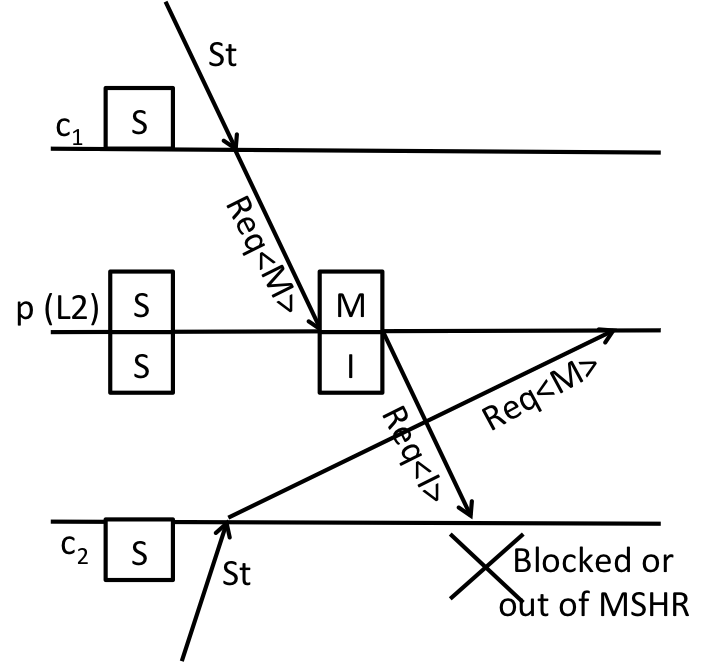
\includegraphics[scale=0.4]{unknown}
\caption{Effect of violating Requirement \ref{cReqNoBlockPReq} (requests blocking responses from parent)}
\label{unknown}
\end{figure}
\floatstyle{boxed}
\restylefloat{figure}

Let's say some request from the core is blocking $c_1$ from receiving the
request. $c_1$ will never respond back to $p$. But $p$ will be waiting in
procedure \dReqL{}, and will never start handling the request from $c_1$. This
will create a deadlock.  The same deadlock is also created when $c_1$ is out of
thread resources to create a thread to handle the downgrade request from $p$.
Figure \ref{unknown} depicts this scenario.

Let's extend this scenario further. Let $c_1$ send a downgrade-to-$I$ response
to $p$. Let's assume that the downgrade-to-$I$ response from $c_1$ is being
blocked. This means $p$ doesn't receive the downgrade-to-$I$ response, leading
to the same deadlock. This is also the same if there isn't a dedicated resource
in $p$ to handle the downgrade response.

\floatstyle{boxed}
\restylefloat{figure}

%The basic ordering requirement is that responses should not overtake each other
%when they are sent from the same source to the same destination. Similarly,
%requests should not overtake responses from the same source to the same
%destination.

\begin{figure}\small
\begin{requirement}
An incoming response for an address $a$ from a child $c$ should not be
received before another incoming response from the same $c$ and the
same $a$ sent earlier has been received\label{cRespFifo}
\end{requirement}
\begin{requirement}
An incoming request for an address $a$ from a source $n$ should not be
received before another incoming response from the same $n$ and the
same $a$ sent earlier has been received\label{reqNoOvertakeResp}
\end{requirement}
\caption{Ordering requirements}
\label{order}
\end{figure}

Figure \ref{order} gives the exact ordering
requirements between messages transmitted between the caches.

We will illustrate the need for Requirements \ref{cRespFifo} and
\ref{reqNoOvertakeResp} using a 2-level cache hierarchy with two L1 caches $c_1$ and
$c_2$, and one shared L2 cache $p$. Each core can have several outstanding
memory requests.

\floatstyle{plain}
\restylefloat{figure}
\begin{figure}
\centering
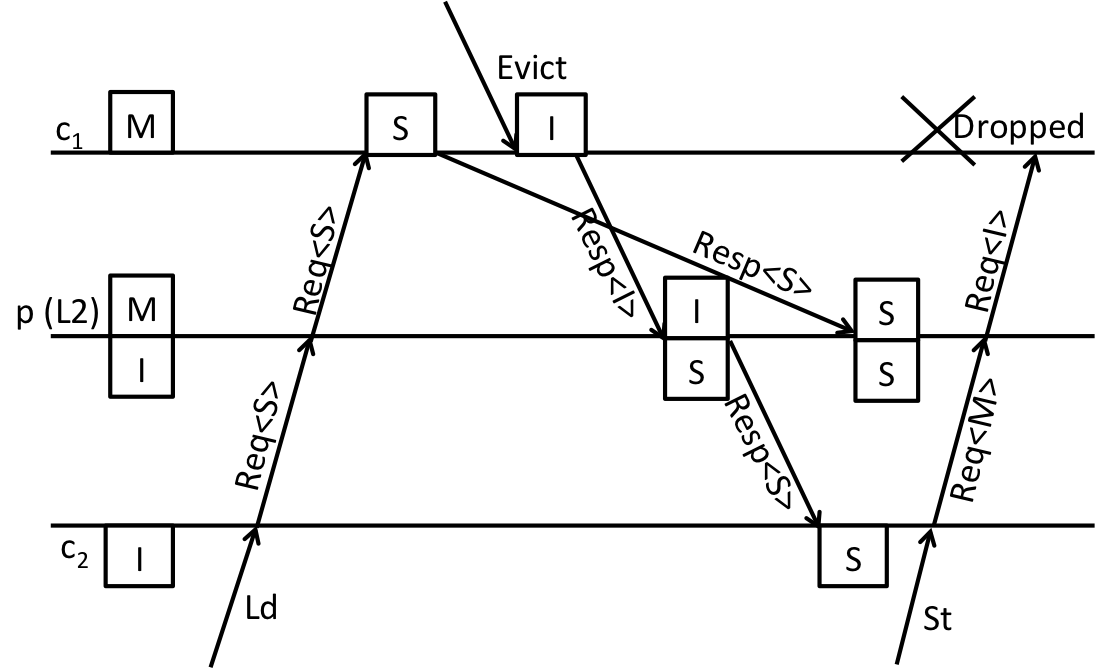
\includegraphics[scale=0.4]{complicated}
\caption{Effect of violating Requirement \ref{cRespFifo} (order between responses)}
\label{complicated}
\end{figure}
\floatstyle{boxed}
\restylefloat{figure}

Let's say $c_1.state[a] = p.dir[c_1][a] = M$, $c_2.state[a] = p.dir[c_2][a] =
I$. $c_2$ gets a load request from its processor for address $a$ and sends an
upgrade request to $p$. $p$ sends a downgrade-to-$S$ request to $c_1$. $c_1$
receives the downgrade-to-$S$ request and downgrades to $S$, sending a downgrade
response to $p$. $c_1$ decides to evict address $a$ to make room for another
address $a'$, because of a request from the core for $a'$ not present in $c_1$.
$c_1$ sends a downgrade-to-$I$ response to $p$. Let's say the second downgrade
to $I$ response reaches $p$ first, violating Requirement \ref{cRespFifo}. $p$
sends an upgrade-to-$S$ response to $c_2$. $c_2$ receives the upgrade response
and changes state to $S$. $p$ then receives the second downgrade-to-$S$ response
from $c_1$, changing its $p.dir[c_1][a]$ to $S$. $c_2$ sends an upgrade-to-$M$
request to $p$ because of a store from its core for $a$. $p$ will send a
downgrade-to-$I$ request to $c_1$, but $c_1$ drops the request as seen in
procedure \dReq{} in Figure \ref{realistic}. So $p$ will never receive a
response from $c_1$ leading to a deadlock. This is illustrated in Figure
\ref{complicated}. In the figure, the timeline moves from left to right.
Whenever the state of the directory or the cache changes, we show the new state.
Messages are shown using arrows from the source to the destination, moving
across time.

\floatstyle{plain}
\restylefloat{figure}
\begin{figure}
\centering
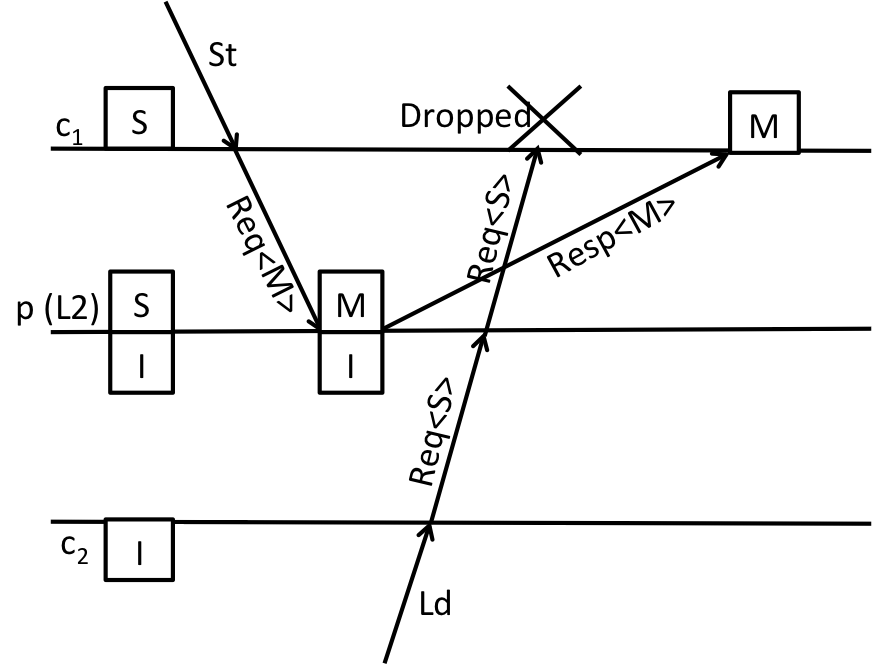
\includegraphics[scale=0.4]{lessComplicated}
\caption{Effect of violating Requirement \ref{reqNoOvertakeResp} (requests overtaking responses)}
\label{lessComplicated}
\end{figure}
\floatstyle{boxed}
\restylefloat{figure}

Consider another scenario starting with $c_1.state[a] = p.dir[c_1][a] = S$ and
$c_2.state[a] = p.dir[c_2][a] = I$. $c_1$ receives a store request and sends an
upgrade-to-$M$ request to $p$. $p$ sends back an upgrade-to-$M$ response to
$c_1$. $c_2$ gets a load request for address $a$ and sends an upgrade-to-$S$
request to $p$. $p$ sends a request to $S$ to $c_1$. Suppose Requirement
\ref{reqNoOvertakeResp} is violated and the request to $S$ reaches $c_1$ before
the response to $M$. $c_1$ will drop the request since its already in state $S$,
and so $p$ will never get a response leading to a deadlock. This is illustrated
in Figure \ref{lessComplicated}.

These scenarios show that these ordering requirements are indeed necessary for a
correct cache coherence protocol.


\subsection{Suspension due to eviction}
A thread can also get suspended if it needs to evict another line because of
lack of space in the cache for the address corresponding to the thread. This is
because, an address that is currently being processed by another thread should
not be evicted. Another point to note is that an address which is already
selected for eviction, but is waiting for the children to downgrade to $I$,
should not be selected for eviction by another address.
